\documentclass[11pt]{article}
\usepackage[margin=1.1in]{geometry}
\usepackage{booktabs}
\usepackage{amsmath}
\usepackage{graphicx}
\usepackage{xcolor}
% Paper chrome matches the UK sister paper (PolicyEngine/uk-ai-study):
% template blue for headings and links, PolicyEngine teal in figures.
\definecolor{paperblue}{rgb}{0,0,0.7}
\definecolor{peteal}{HTML}{39C6C0}
\usepackage{sectsty}
\allsectionsfont{\color{paperblue}}
\usepackage[colorlinks=true, citecolor=paperblue, linkcolor=paperblue, urlcolor=paperblue]{hyperref}
\usepackage[hang,flushmargin]{footmisc}
\usepackage{natbib}
\bibliographystyle{apalike}
% values_generated.tex — machine-generated by analysis/emit_paper_values.py
% from analysis/outputs/ai_scenarios.json, src/data/shiftSweepData.json and
% analysis/outputs/yale_publishable_2030.xlsx. DO NOT EDIT BY HAND.
\newcommand{\genBaselinePovertyPct}{12.13}
\newcommand{\genBaselineGini}{0.4625}
\newcommand{\genRapidFixedRev}{+581}
\newcommand{\genRapidPropRev}{+211}
\newcommand{\genRapidExpRev}{+244}
\newcommand{\genRapidCompRev}{+179}
\newcommand{\genRapidShareKeptPct}{36}
\newcommand{\genRapidFixedPovPp}{-1.09}
\newcommand{\genRapidPropPovPp}{+0.11}
\newcommand{\genRapidCompPovPp}{-1.54}
\newcommand{\genRapidExpPovPp}{+1.72}
\newcommand{\genRapidPovSpanPp}{3.26}
\newcommand{\genRapidRevRelMovePct}{36}
\newcommand{\genRapidCompLambda}{0.928}
\newcommand{\genRapidExpLambda}{1.072}
\newcommand{\genRapidCompCrossover}{118,287}
\newcommand{\genRapidExpCrossover}{168,205}
\newcommand{\genSSCap}{214,200}
\newcommand{\genShareWagesAboveCapPct}{15.8}
\newcommand{\genShareWorkersAboveCapPct}{5.7}
\newcommand{\genModelledLaborShareT}{15.9}
\newcommand{\genModelledCapitalShareT}{5.3}
\newcommand{\genRapidCompPayroll}{+34}
\newcommand{\genRapidPropPayroll}{-16}
\newcommand{\genRapidExpPayroll}{-70}
\newcommand{\genRapidCompLaborPct}{-0.94}
\newcommand{\genGrossTaxSwing}{122}
\newcommand{\genTransferSwing}{57}
\newcommand{\genTransferAbsorbPct}{47}
\newcommand{\genBenefitSwing}{42}
\newcommand{\genRapidCompBenefits}{-20}
\newcommand{\genRapidExpBenefits}{+22}
\newcommand{\genSnapSwing}{19}
\newcommand{\genRapidCompSnap}{-9}
\newcommand{\genRapidExpSnap}{+10}
\newcommand{\genSsiSwing}{3}
\newcommand{\genCreditSwing}{15}
\newcommand{\genModCompBenefits}{-11}
\newcommand{\genModExpBenefits}{+8}
\newcommand{\genNetRevSwing}{65}
\newcommand{\genRapidCompState}{+24}
\newcommand{\genRapidPropState}{+36}
\newcommand{\genRapidExpState}{+48}
\newcommand{\genRapidExpStateNet}{+47}
\newcommand{\genStateTopFiveSharePct}{56}
\newcommand{\genStateFirst}{CA +10.0}
\newcommand{\genStateSecond}{NY +5.8}
\newcommand{\genStateThird}{NJ +1.6}
\newcommand{\genStateFourth}{MA +1.3}
\newcommand{\genStateFifth}{MD +1.2}
\newcommand{\genWAState}{+1.1}
\newcommand{\genNZeroStates}{7}
\newcommand{\genRealZeroRev}{-61}
\newcommand{\genRealFullRev}{+211}
\newcommand{\genRealBreakevenPct}{22.5}
\newcommand{\genRealPovMinPct}{12.24}
\newcommand{\genRealPovMaxPct}{12.27}
\newcommand{\genTheirRapidCit}{+84}
\newcommand{\genRealZeroAllIn}{+23}
\newcommand{\genSlowScopeFull}{+6}
\newcommand{\genSlowScopeExcl}{-4}
\newcommand{\genModScopeFull}{+144}
\newcommand{\genModScopeExcl}{+98}
\newcommand{\genRapidScopeFull}{+211}
\newcommand{\genRapidScopeExcl}{+106}
\newcommand{\genRapidScopeDiff}{-105}
\newcommand{\genRapidPropMarketDelta}{+760}
\newcommand{\genRapidPropATRPct}{27.8}
\newcommand{\genBridgeOursIIT}{+287}
\newcommand{\genBridgeOursPayroll}{-70}
\newcommand{\genBridgeWedge}{+84}
\newcommand{\genBridgeOursTotal}{+301}
\newcommand{\genBridgeTheirsIIT}{+195}
\newcommand{\genBridgeTheirsPayroll}{-63}
\newcommand{\genBridgeTheirsTotal}{+216}
\newcommand{\genBridgeRatio}{1.40}
\newcommand{\genBridgeOursCboPct}{4.6}
\newcommand{\genBridgeTheirsCboPct}{3.3}
\newcommand{\genIITRatio}{1.47}
\newcommand{\genIITRatioProp}{1.97}
\newcommand{\genPayrollTripletOurs}{+34/-16/-70}
\newcommand{\genPayrollTripletTheirs}{+37/-11/-63}
\newcommand{\genTiltTheirsSlow}{3.62}
\newcommand{\genTiltOursMatchedSlow}{3.13}
\newcommand{\genTiltOursHouseholdSlow}{7.29}
\newcommand{\genTiltTheirsMod}{1.71}
\newcommand{\genTiltOursMatchedMod}{1.65}
\newcommand{\genTiltOursHouseholdMod}{2.01}
\newcommand{\genTiltTheirsRapid}{2.11}
\newcommand{\genTiltOursMatchedRapid}{2.00}
\newcommand{\genTiltOursHouseholdRapid}{2.75}
\newcommand{\genSlowCompTheirsLowerPct}{84}
\newcommand{\genSlowCompOursLowerPct}{93}
\newcommand{\genSweepYear}{2026}
\newcommand{\genSweepBaseGini}{0.470}
\newcommand{\genSweepFullGini}{0.768}
\newcommand{\genSweepBasePovPct}{13.2}
\newcommand{\genSweepFullPovPct}{61.2}
\newcommand{\genSweepTroughRev}{-880}
\newcommand{\genSweepTroughShift}{90}
\newcommand{\genSweepFullRev}{-790}
\newcommand{\genSweepLaborT}{12.4}
\newcommand{\genSweepCapitalT}{2.7}
\newcommand{\genSweepHHCapSharePct}{51}
\newcommand{\genSweepTopDecilePct}{+58}
\newcommand{\genSweepWorstDecilePct}{-48.5}
\newcommand{\genSweepWorstDecile}{5}
\newcommand{\genForecastShiftSlowPct}{0.9}
\newcommand{\genForecastShiftModPct}{3.1}
\newcommand{\genForecastShiftRapidPct}{7.6}
\newcommand{\genIdentityMaxResidual}{0.000}
\newcommand{\genLaborTargetMaxErr}{2e-16}
\newcommand{\genModelVersion}{1.764.6}
\newcommand{\genRunnerVersion}{5.0.1}
\newcommand{\genDataBuild}{populace-us-2024-buildp-sparse-rmloss100-cae8640-20260728T011454Z}
 % machine-generated numeric macros from run outputs
% tables_generated.tex — machine-generated by analysis/emit_paper_values.py.
% DO NOT EDIT BY HAND.
\newcommand{\tabScenarioGrid}{%
\begin{tabular}{lrrrrrrr}
\toprule
Scenario & Revenue & Income tax & Payroll & State & Poverty & $\Delta$pp & Net Gini \\
\midrule
Slow / shares fixed & +47 & +29 & +10 & +6 & 11.99\% & -0.14 & 0.4627 \\
Slow / compressive & +3 & +3 & -1 & +1 & 12.01\% & -0.12 & 0.4622 \\
Slow / proportional & +6 & +11 & -5 & +2 & 12.17\% & +0.04 & 0.4632 \\
Slow / expansive & +10 & +19 & -10 & +3 & 12.33\% & +0.20 & 0.4643 \\
\addlinespace
Moderate / shares fixed & +289 & +178 & +61 & +35 & 11.46\% & -0.67 & 0.4640 \\
Moderate / compressive & +128 & +65 & +33 & +15 & 11.18\% & -0.95 & 0.4596 \\
Moderate / proportional & +144 & +114 & +7 & +21 & 12.00\% & -0.13 & 0.4656 \\
Moderate / expansive & +163 & +164 & -20 & +28 & 12.84\% & +0.71 & 0.4718 \\
\addlinespace
Rapid / shares fixed & +581 & +358 & +121 & +71 & 11.04\% & -1.09 & 0.4654 \\
Rapid / compressive & +179 & +98 & +34 & +24 & 10.59\% & -1.54 & 0.4581 \\
Rapid / proportional & +211 & +193 & -16 & +36 & 12.24\% & +0.11 & 0.4699 \\
Rapid / expansive & +244 & +294 & -70 & +48 & 13.85\% & +1.72 & 0.4820 \\
\bottomrule
\end{tabular}}
\newcommand{\tabTilt}{%
\begin{tabular}{lrrr}
\toprule
Scenario & Shares fixed & As forecast & Share kept \\
\midrule
Slow & +47 & +6 & 14\% \\
Moderate & +289 & +144 & 50\% \\
Rapid & +581 & +211 & 36\% \\
\bottomrule
\end{tabular}}
\newcommand{\tabRealization}{%
\begin{tabular}{lr}
\toprule
Realized share & Revenue \\
\midrule
0\% & -61 \\
25\% & +7 \\
50\% & +74 \\
75\% & +142 \\
100\% (their assumption) & +211 \\
\bottomrule
\end{tabular}}
\newcommand{\tabCapitalScope}{%
\begin{tabular}{lrrr}
\toprule
Scenario & Full capital set & Excl.\ retirement & Difference \\
\midrule
Slow & +6 & -4 & -10 \\
Moderate & +144 & +98 & -46 \\
Rapid & +211 & +106 & -105 \\
\bottomrule
\end{tabular}}
\newcommand{\tabBridge}{%
\begin{tabular}{lrrrr}
\toprule
Rapid / expansive & IIT (net) & Payroll & Corporate wedge & Total \\
\midrule
This paper & +287 & -70 & +84 & +301 \\
Budget Lab & +195 & -63 & +84 & +216 \\
\bottomrule
\end{tabular}}
\newcommand{\tabPayrollCells}{%
\begin{tabular}{lrrrr}
\toprule
Rapid variant & \multicolumn{2}{c}{IIT net of credits} & \multicolumn{2}{c}{Payroll} \\
 & Ours & Theirs & Ours & Theirs \\
\midrule
Compressive & +104 & +11 & +34 & +37 \\
Proportional & +193 & +98 & -16 & -11 \\
Expansive & +287 & +195 & -70 & -63 \\
\bottomrule
\end{tabular}}
\newcommand{\tabStates}{%
\begin{tabular}{lr}
\toprule
State & Net revenue change \\
\midrule
CA & +10.01 \\
NY & +5.82 \\
NJ & +1.58 \\
MA & +1.33 \\
MD & +1.16 \\
VA & +1.15 \\
WA & +1.13 \\
MN & +1.02 \\
IL & +0.91 \\
OR & +0.89 \\
\addlinespace
\multicolumn{2}{l}{\footnotesize 7 states collect exactly \$0: FL, NV, NH, SD, TN, TX, WY.} \\
\bottomrule
\end{tabular}}
\newcommand{\tabSweep}{%
\begin{tabular}{rrrrr}
\toprule
Shift & Revenue & Income tax & Poverty & Net Gini \\
\midrule
0\% & +0 & +0 & 13.2\% & 0.470 \\
10\% & -135 & +44 & 15.0\% & 0.490 \\
20\% & -255 & +101 & 16.9\% & 0.513 \\
30\% & -370 & +176 & 20.1\% & 0.536 \\
40\% & -486 & +265 & 23.9\% & 0.561 \\
50\% & -592 & +371 & 29.3\% & 0.588 \\
60\% & -688 & +493 & 35.4\% & 0.617 \\
70\% & -773 & +638 & 43.1\% & 0.647 \\
80\% & -847 & +807 & 50.7\% & 0.681 \\
90\% & -880 & +1000 & 57.6\% & 0.719 \\
100\% & -790 & +1235 & 61.2\% & 0.768 \\
\bottomrule
\end{tabular}}
 % machine-generated tables from run outputs

\title{\bfseries What if income shifts from labor to capital?\\[0.15cm]
The fiscal and distributional incidence of AI-driven growth in the United
States\thanks{\textbf{Acknowledgements:} the cell-level reconciliation in
Section~\ref{sec:reconciliation} is possible because the Budget Lab at Yale
publishes its code and complete result grids alongside its reports; I thank
them for that practice. All errors are mine. An interactive companion to this
paper is at
\href{https://policyengine.org/us/ai-inequality/income-shift}{policyengine.org/us/ai-inequality/income-shift};
code and data references are in Appendix~\ref{app:repro}.}\\[0.7cm]}
\author{Max Ghenis\thanks{PolicyEngine. Email:
\href{mailto:max@policyengine.org}{max@policyengine.org}.}}
\date{\small \ifcase\month\or January\or February\or March\or April\or May\or
June\or July\or August\or September\or October\or November\or December\fi\
\the\year}

\begin{document}
\maketitle

\begin{abstract}
\noindent I study how AI-driven growth would move United States government
revenue, benefit outlays, poverty and inequality, by running two experiment
families through PolicyEngine-US, an open-source static microsimulation of the
full federal and state tax and transfer system, on openly published microdata.
A mechanism sweep shifts 0--100\% of labor income into capital income under
current law; a scenario set adopts the Budget Lab's calibration of the
\citet{karger2026} forecaster survey --- Slow, Moderate and Rapid adoption
crossed with three wage-inequality variants --- so that remaining differences
between the two models are differences in coverage, not assumptions. In Rapid,
the forecast tilt toward capital keeps \genRapidShareKeptPct\% of the revenue
gain that shares-fixed growth would deliver (\genRapidPropRev B against
\genRapidFixedRev B) and erases the poverty gain from growth
(\genRapidFixedPovPp pp becomes \genRapidPropPovPp pp). Across the
wage-inequality variants, net revenue stays within
\genRapidCompRev B--\genRapidExpRev B while the poverty outcome flips sign,
from \genRapidCompPovPp pp to \genRapidExpPovPp pp; automatic transfer
responses absorb \genTransferAbsorbPct\% of the gross-tax swing across those
variants, \$\genBenefitSwing B of it in programs outside a tax-only model, and
state tax doubles from \genRapidCompState B to \genRapidExpState B. If less
than \genRealBreakevenPct\% of the incremental capital income is realized on
tax returns, the household sector loses revenue on Rapid AI growth.
Reconciled cell by cell against the Budget Lab's published grid, payroll
responses agree closely throughout, while the bridged headline is
\genBridgeOursTotal B against their \genBridgeTheirsTotal B
(\genBridgeRatio$\times$), concentrated in the income-tax response to the
capital shock.
\end{abstract}

\medskip
\noindent\textbf{Keywords:} artificial intelligence, factor shares,
microsimulation, taxation, transfers, poverty, inequality, state taxes

\medskip
\noindent\textbf{JEL codes:} H24, H53, H71, D31, I32, O33, C63

\newpage
\input{sections/intro}
\section{Related work}\label{sec:literature}

The paper sits at the intersection of three literatures: macro-fiscal
analyses of AI, tax-benefit microsimulation of technology shocks, and the
factor-share literature that motivates the experiment's central mechanism.

\textbf{AI and the public finances.} \citet{iselinnunn2026} is the direct
antecedent: they translate the \citet{karger2026} forecaster survey into
2030 growth, factor-share and wage-distribution scenarios and score them
through a federal individual income and payroll tax microsimulation built on
the IRS Public Use File, adding a corporate revenue wedge outside the
microsimulation. Their central finding --- that growth accruing to capital
raises less revenue than the same growth at fixed factor shares, by roughly a
factor of two in the Rapid scenario --- is the claim this paper re-derives on
independent machinery and extends to transfers, poverty and states.
\citet{karger2026} elicit forecasts from economists, AI-company staff, policy
researchers, superforecasters and the public; the median expects modest
GDP acceleration by 2030 with substantial disagreement about wage
distribution effects --- disagreement this paper propagates rather than
resolves. \citet{acemoglu2025} argues on task-level grounds for modest
aggregate effects; \citet{bastani2024} survey the tax-design questions AI
raises, including whether existing bases can reach AI-driven rents.

\textbf{Microsimulation of AI shocks.} Closest in method are two companion
studies on European systems. \citet{doorley2026} run scenario-based AI
employment and wage shocks through the Irish SWITCH model, and
\citet{ahmadi2026} runs occupation-level exposure-based displacement, wage and
capital shocks through PolicyEngine UK, treating the incidence of
displacement as an explicit scenario axis. This paper is the United States
member of that family, but it differs in the shock design: rather than
displacement incidence, it varies the factor composition and
wage-distribution shape of income growth, matching the Budget Lab's
calibration to enable the cell-level reconciliation of
Section~\ref{sec:reconciliation}. Occupation-level exposure measures
\citep{felten2021, eloundou2024} are the natural next refinement of the wage
channel here, as Section~\ref{sec:discussion} discusses; both this paper's
repository and the Budget Lab's roadmap point the same direction.

\textbf{Factor shares and automation.} The premise that technology can move
income between labor and capital at scale is not hypothetical: the global
decline of the labor share is documented by \citet{karabarbounisneiman2014},
and \citet{acemoglurestrepo2018} provide the task-model mechanics by which
automation reallocates value added from labor to capital. What
microsimulation adds to that literature is the statutory detail: a dollar
moved from wages to capital income changes its withholding, its marginal
rate schedule, its payroll treatment, its state treatment, and the transfer
payments of the household it leaves --- none of which aggregate models
carry. The scenarios here take the CBO baseline as the no-AI counterfactual,
using the same February 2026 projections the Budget Lab anchors to
\citep{cbo2026}.

\section{Model, data, and experiment designs}\label{sec:method}

\subsection{Model and data}

All results come from PolicyEngine-US version \genModelVersion{}, an
open-source static microsimulation of United States federal and state tax and
benefit law, executed through the \texttt{policyengine.py} runtime
(version \genRunnerVersion{}), which certifies the pairing of model version
and dataset build. The dataset is \texttt{populace-us} build
\texttt{cae8640} (28 July 2026), an openly published enhanced-CPS microdata
file for 2024, uprated by the model to the analysis years. The mechanism
sweep of Section~\ref{sec:sweep} is run at \genSweepYear{}; the calibrated
scenarios are run at 2030, matching the Budget Lab's horizon. In the 2030
baseline, SPM poverty is \genBaselinePovertyPct\% and the household
net-income Gini is \genBaselineGini{} (household-level, unequivalized;
Section~\ref{sec:discussion} discusses comparability).

The model covers federal individual income tax (including capital gains
rates, the net investment income tax and the alternative minimum tax),
payroll taxes on both employee and employer sides plus self-employment tax,
refundable credits (EITC, refundable CTC and others), the major means-tested
transfer programs (SNAP, SSI, TANF, WIC, school meals, housing subsidies,
broadband subsidies), and the tax and benefit codes of all fifty states and
DC. Health programs (Medicaid, CHIP, ACA subsidies) are valued in the model
but excluded from net-income accounting in these runs by the model's default
simulation switch, so no result here contains a health-program response in
either direction. Everything is static: no labor supply, behavioral,
avoidance or enforcement responses, matching the Budget Lab's individual
microsimulation.

\textbf{Accounting.} Net government revenue is defined as taxes minus
transfers: household tax before refundable credits (federal and state,
including employee-side payroll) plus employer payroll tax, minus refundable
credits and benefit outlays. An identity check --- the change in market
income minus the change in household net income must equal the household-side
revenue change --- closes to \$\genIdentityMaxResidual B in every scenario.
Where the paper compares against the Budget Lab
(Section~\ref{sec:reconciliation}), it restates results on their narrower
basis: federal individual income tax net of refundable credits, plus payroll.

\subsection{Design I: the mechanism sweep}\label{sec:method-sweep}

The sweep isolates composition. In 10-point steps from 0\% to 100\%, it
reduces every person's positive employment and self-employment income by the
step share and redistributes the same weighted total to positive capital
income in proportion to existing holdings, holding modelled market income
fixed. The \genSweepYear{} baseline contains \$\genSweepLaborT T of positive
labor income and \$\genSweepCapitalT T of positive capital income, with
\genSweepHHCapSharePct\% of households receiving any positive capital income
--- so the sweep concentrates income by construction, and the question is
what current law does about it.

The sweep's limitation is deliberate: a pure reallocation holds output fixed,
while forecasters expect AI to raise output \emph{and} tilt its composition.
The sweep therefore answers ``what does composition alone do to current
law?'', and the calibrated scenarios answer ``what happens on the paths
forecasters actually expect?''. The two connect through a
forecast-equivalence mapping: the share of baseline labor income that the
tilt removes, $k = 1 - (1+g_L)/(1+g_Y)$, places each scenario on the sweep
axis at \genForecastShiftSlowPct\% (Slow), \genForecastShiftModPct\%
(Moderate) and \genForecastShiftRapidPct\% (Rapid) --- the sweep's
forecast-relevant range is its first decade, and the rest is out-of-sample
stress test.

\subsection{Design II: forecaster-calibrated scenarios}\label{sec:method-scenarios}

The scenarios adopt the Budget Lab's calibration of \citet{karger2026}
exactly. Each scenario is defined by an annual real GDP growth rate under AI
(Slow 2.0\%, Moderate 2.6\%, Rapid 3.3\%) and a 2030 labor share of factor
income (55.0\%, 53.8\%, 51.3\%). Growth is expressed in excess of the CBO
baseline path: the five-year output shock is
$g_Y = (1+r_{\mathrm{ai}})^5 / G_{\mathrm{CBO}} - 1$, and the factor shocks
follow from the target shares,
\begin{equation}
g_K = \frac{\theta^1_K (1+g_Y) - \theta^0_K}{\theta^0_K}, \qquad
g_L = \frac{\theta^1_L (1+g_Y) - \theta^0_L}{\theta^0_L}.
\end{equation}
Two inputs their report uses but does not print --- the cumulative CBO
baseline factor $G_{\mathrm{CBO}} = 1.0976$ and the pre-shock labor share
$\theta^0_L = 0.5550$ --- are recovered by inverting their published
formulas against the nine derived values in their Table~1; unit tests
reproduce all nine to within 0.005\,pp and re-derive the labor share by grid
search so the constants cannot drift.

The wage-inequality channel is their stylization $\lambda = 1 \pm g_Y$: a
spread transform on log labor income,
$\ln Y^1_i = \mu^1 + \lambda\,(\ln Y^0_i - \mu^0)$, equivalently
$Y^1_i = C\,Y_i^{0\,\lambda}$ with $C$ in closed form, with the aggregate
pinned to $(1+g_L)$ times baseline. Compressive ($\lambda<1$) narrows the
wage distribution around the same aggregate; expansive ($\lambda>1$) widens
it; proportional scales every wage equally. The transform is applied at the
person level because the payroll result turns on a per-person threshold, the
Social Security taxable maximum (\$\genSSCap{} in 2030; at baseline
\genShareWagesAboveCapPct\% of wage income and
\genShareWorkersAboveCapPct\% of workers sit above it).

The capital shock scales nine capital income variables --- long- and
short-term capital gains, taxable interest, qualified and non-qualified
dividends, rental income, partnership and S-corporation income, taxable
pension income and taxable IRA distributions --- in proportion to existing
holdings, after routing pass-through income through the Budget Lab's
labor/capital split rule. Appendix~\ref{app:routing} traces every shocked
variable into IRS gross income and household market income, confirming the
shock reaches the tax base rather than being recomputed away; the labor
aggregate lands on its target to within relative error
\genLaborTargetMaxErr{}. Each scenario also has a shares-fixed
counterfactual growing both factors at $g_Y$, the comparison behind the
Budget Lab's ``roughly twice as large'' finding.

Two further axes vary definitional assumptions their report flags. A
\emph{realization rate} routes a fraction of the incremental capital flow
outside the taxable base (their assumption corresponds to 1.0); and a
\emph{capital-scope} variant excludes taxable pension income and IRA
distributions from the capital set, since those are taxed at ordinary rates
and their inclusion works against the ``capital is taxed lightly''
mechanism.

\section{Results}\label{sec:results}

\subsection{The mechanism at full range}\label{sec:sweep}

Figure~\ref{fig:sweep-rev} runs the composition mechanism from 0\% to 100\%.
Net government revenue falls almost monotonically as labor income becomes
capital income, bottoming at \genSweepTroughRev B at a
\genSweepTroughShift\% shift: the income tax initially loses progressivity
revenue as wages leave the schedule, payroll revenue falls roughly linearly
with the wage base, state codes track the federal pattern, and benefit
outlays rise as wage-dependent households qualify for means-tested support.
The distributional counterpart (Figure~\ref{fig:sweep-dist}) is severe by
construction --- only \genSweepHHCapSharePct\% of households hold any
positive capital income, so the net-income Gini rises from
\genSweepBaseGini{} to \genSweepFullGini{} and SPM poverty from
\genSweepBasePovPct\% to \genSweepFullPovPct\% at the full shift, with the
top decile's mean net income rising \genSweepTopDecilePct\% while decile
\genSweepWorstDecile{} falls \genSweepWorstDecilePct\%. The
forecast-equivalent range --- the shaded band at
\genForecastShiftSlowPct{}--\genForecastShiftRapidPct\% --- says how much of
this axis the 2030 forecasts actually reach: the first decade. The sweep's
value is the mechanism it exposes, not the tail.

\begin{figure}[t]
\centering
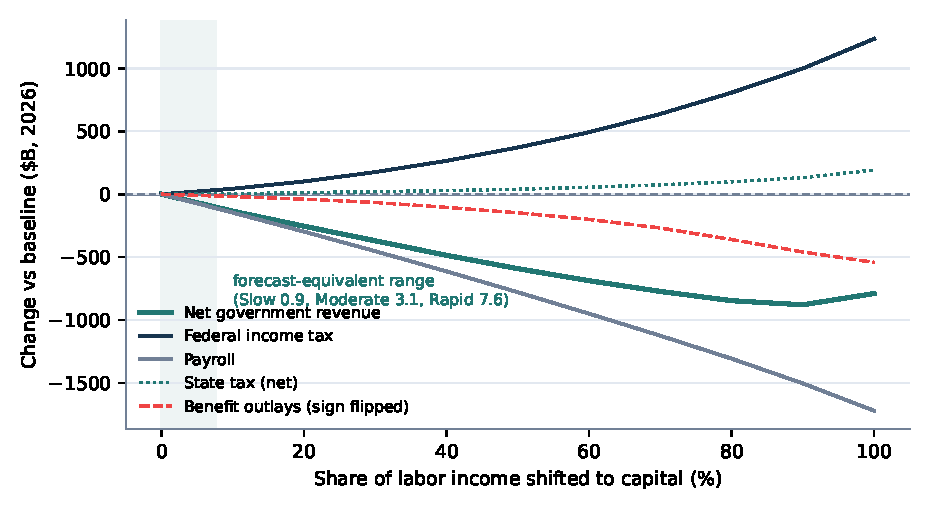
\includegraphics[width=0.92\textwidth]{figures/sweep_revenue.pdf}
\caption{Revenue under a 0--100\% labor-to-capital shift,
\genSweepYear{}. Lines are changes against baseline; benefit outlays are
sign-flipped so a rising line is a fiscal cost. The shaded band marks the
forecast-equivalent positions of the 2030 scenarios.}
\label{fig:sweep-rev}
\end{figure}

\begin{figure}[t]
\centering
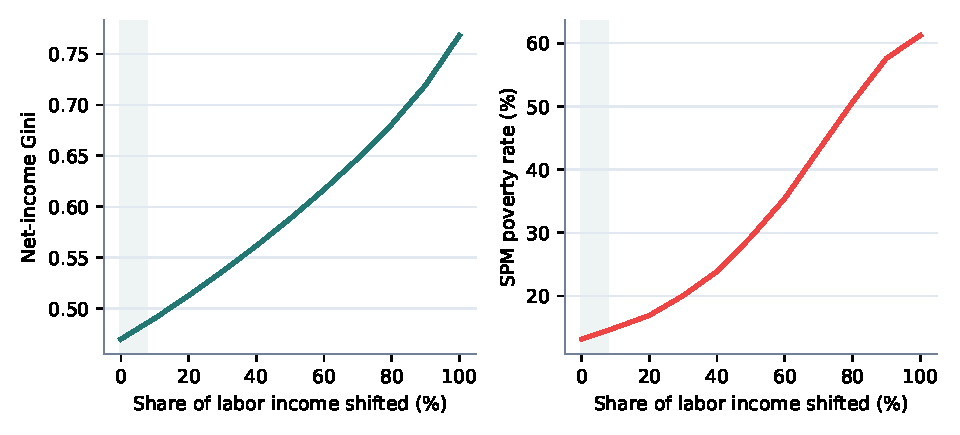
\includegraphics[width=0.92\textwidth]{figures/sweep_distribution.pdf}
\caption{Inequality and poverty under the same sweep.}
\label{fig:sweep-dist}
\end{figure}

\subsection{Calibrated scenarios}\label{sec:scenarios}

Table~\ref{tab:grid} reports all twelve scenario cells at 2030 against the
same-year current-law baseline; Figure~\ref{fig:scenarios} plots the Rapid
pattern. Two published Budget Lab mechanisms reproduce on independent
machinery. Within each scenario, moving from compressive to expansive raises
income-tax revenue through progressivity and lowers payroll revenue as
earnings cross the Social Security taxable maximum. And the tilt is
expensive: Table~\ref{tab:tilt} shows each scenario keeping a fraction of its
shares-fixed revenue --- \genRapidShareKeptPct\% in Rapid
(\genRapidPropRev B against \genRapidFixedRev B).

\begin{table}[t]
\centering
\small
\tabScenarioGrid
\caption{Scenario grid, 2030, \$B change against the current-law baseline
(SPM poverty \genBaselinePovertyPct\%, net Gini \genBaselineGini{}).
``Revenue'' is net government revenue (federal and state taxes minus
refundable credits and benefits); ``Income tax'' is federal income tax
gross of refundable credits; ``State'' is state tax before refundable state
credits.}
\label{tab:grid}
\end{table}

\begin{table}[t]
\centering
\tabTilt
\caption{What the tilt toward capital costs: net revenue with factor shares
fixed versus as forecast (proportional wage spread), \$B, 2030.}
\label{tab:tilt}
\end{table}

\begin{figure}[t]
\centering
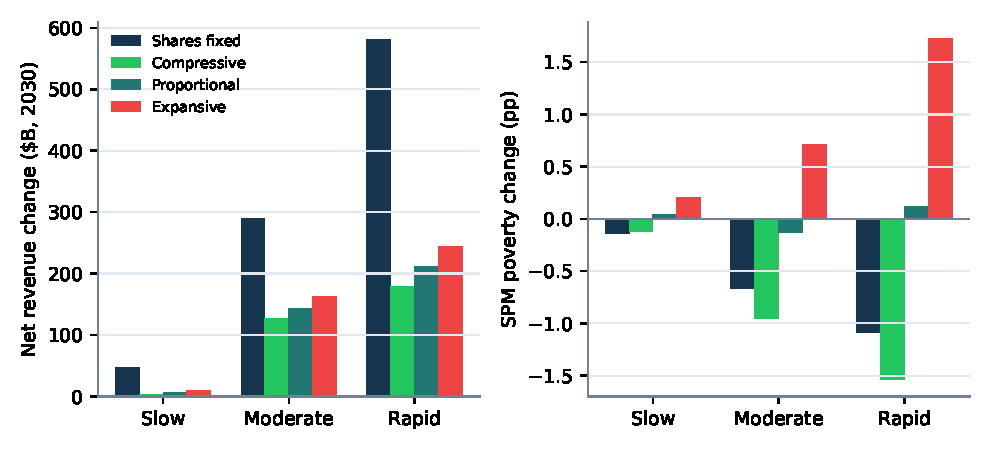
\includegraphics[width=0.95\textwidth]{figures/scenarios.pdf}
\caption{Net revenue (left) and SPM poverty change (right) by scenario and
wage-inequality variant, 2030.}
\label{fig:scenarios}
\end{figure}

The payroll-cap mechanism runs in both directions, which is worth stating
because it is easy to get backwards: under Rapid~/~compressive, aggregate
labor income \emph{falls} \genRapidCompLaborPct\% and payroll receipts still
\emph{rise} \genRapidCompPayroll B, because compression moves earnings from
above the taxable maximum to below it; under expansive the same cap turns
wage growth into a payroll loss of \genRapidExpPayroll B. The wage-spread
parameter also has a direct household reading: each variant has a crossover
wage below which workers lose (expansive,
\$\genRapidExpCrossover{}) or gain (compressive,
\$\genRapidCompCrossover{}), so under Rapid~/~expansive the great majority of
workers sit on the losing side of a scenario that adds \genRapidExpRev B to
net revenue.

\subsection{The transfer system}\label{sec:transfers}

The Revenue column of Table~\ref{tab:grid} nets transfers out; pulling them
apart shows the safety net responding exactly as designed
(Figure~\ref{fig:transfers}). Across the Rapid wage-spread variants ---
identical aggregate labor income, only its distribution varies --- gross tax
collections swing \$\genGrossTaxSwing B, and automatic transfer responses
absorb \$\genTransferSwing B of that swing, \genTransferAbsorbPct\%.
Non-credit transfers alone swing \$\genBenefitSwing B: \genRapidCompBenefits
B under compressive, as rising low-end wages float households off
means-tested programs, to \genRapidExpBenefits B under expansive as falling
ones push them on. SNAP carries \$\genSnapSwing B of the swing
(\genRapidCompSnap B to \genRapidExpSnap B) and SSI \$\genSsiSwing B;
Moderate shows the same shape (\genModCompBenefits B to \genModExpBenefits
B). Refundable credits contribute the remaining \$\genCreditSwing B --- a
response the Budget Lab's accounting does capture through its tax-credit
outlays line. The \$\genBenefitSwing B of program spending is the piece
outside their model's coverage, and it is the outlay half of the
\genRapidPovSpanPp pp poverty span: the same variant uncertainty their
report scores as a revenue question arrives at households as a benefits
question.

\begin{figure}[t]
\centering
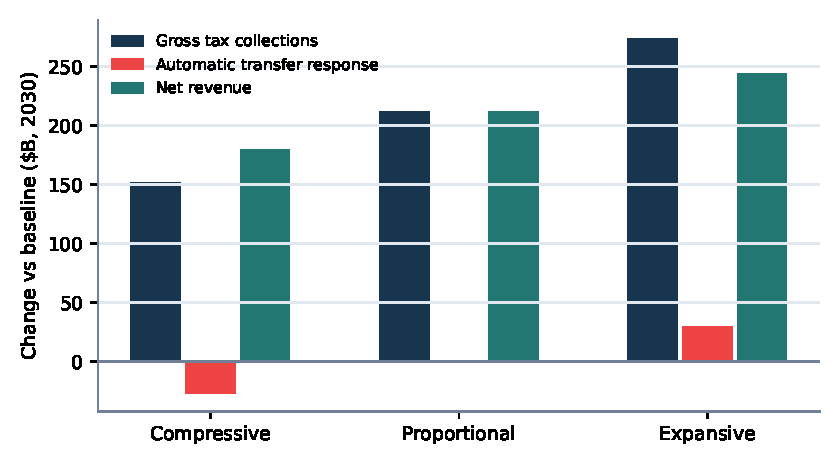
\includegraphics[width=0.8\textwidth]{figures/transfers.pdf}
\caption{Gross tax collections, automatic transfer response, and net revenue
across the Rapid wage-inequality variants, 2030. Transfers (refundable
credits plus benefits) rise exactly when workers lose, absorbing
\genTransferAbsorbPct\% of the gross-tax swing across the variants.}
\label{fig:transfers}
\end{figure}

\subsection{States}\label{sec:states}

State codes are the other channel a federal model does not carry. Under
Rapid~/~proportional they collect \genRapidPropState B, and the state take
doubles across the wage-spread variants (\genRapidCompState B to
\genRapidExpState B) as progressive state schedules concentrate collections
at the top the way federal brackets do. On the Rapid~/~expansive cell used
for the reconciliation below, state tax net of refundable state credits adds
\genRapidExpStateNet B --- roughly a sixth on top of the bridged federal
take.

The geography is concentrated (Figure~\ref{fig:states}): the top five states
collect \genStateTopFiveSharePct\% of the national state take
(\genStateFirst, \genStateSecond, \genStateThird, \genStateFourth,
\genStateFifth, in \$B). \genNZeroStates{} states collect exactly nothing
from the capital shock --- Florida, Nevada, New Hampshire, South Dakota,
Tennessee, Texas and Wyoming --- and Washington is the instructive
exception: it has no income tax either, but its capital-gains excise tax
collects \genWAState B, more than the seven zero-collecting states combined.
A state that taxes capital gains participates in an AI capital boom; a state
that taxes only wages does not participate in an economy where wages are the
shrinking share. State-funded benefit responses are negligible in these runs
(the model's state-benefit registry covers state SSI supplements and
child-care subsidies), so the automatic-stabilizer response above is almost
entirely federal.

\begin{figure}[t]
\centering
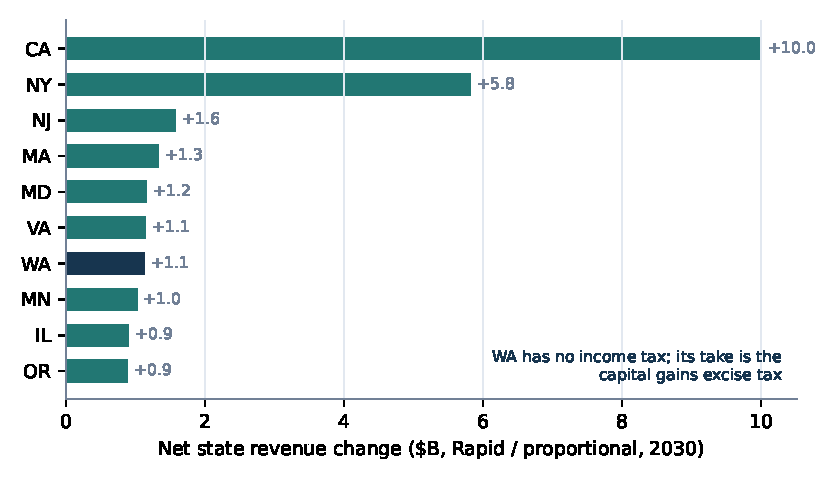
\includegraphics[width=0.8\textwidth]{figures/states.pdf}
\caption{Top ten states by net state revenue change, Rapid~/~proportional,
2030.}
\label{fig:states}
\end{figure}

\section{The two assumptions that dominate}\label{sec:sensitivity}

\subsection{Realization}\label{sec:realization}

The Budget Lab's capital shock assumes AI leaves the realized share of
capital income unchanged, and they flag the assumption as a limitation.
It carries real weight: unrealized gains, retained earnings and accruals
inside retirement accounts never reach the individual tax base. Holding
Rapid~/~proportional fixed and varying only how much of the incremental
capital flow lands on a tax return (Figure~\ref{fig:realization},
Table~\ref{tab:realization} in the appendix), revenue runs from
\genRealZeroRev B at a 0\% realized share to \genRealFullRev B at their
100\% assumption --- linear to within a percent, with breakeven at a
\genRealBreakevenPct\% realized share. Below that, the household side of the
fiscal system loses money on Rapid AI growth: labor income still falls, and
not enough taxable capital income reaches returns to offset it.

One counterweight sits outside the household sector: corporate tax is levied
upstream of household realization, so the Budget Lab's corporate wedge would
still collect about \genTheirRapidCit B on the same shock regardless of the
realized share --- enough to keep the all-in federal total positive, about
\genRealZeroAllIn B, even at the 0\% floor. Low realization shifts the
fiscal burden of an AI boom onto the corporate side; it does not eliminate
it.

Poverty is flat across the entire sweep, between \genRealPovMinPct\% and
\genRealPovMaxPct\%. Whether AI's capital gains are taxable moves the
federal balance sheet by more than a quarter-trillion dollars and moves poor
households essentially not at all: the transfer system responds to what
happens to wages, not to how much of the capital gain the tax system
reaches.

\begin{figure}[t]
\centering
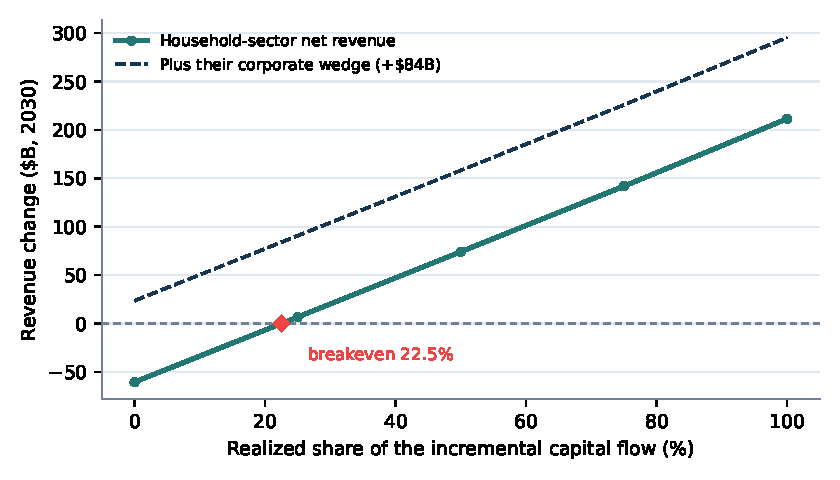
\includegraphics[width=0.8\textwidth]{figures/realization.pdf}
\caption{Net revenue under Rapid~/~proportional as the realized share of the
incremental capital flow varies. The dashed line adds the Budget Lab's
realization-independent corporate wedge.}
\label{fig:realization}
\end{figure}

\subsection{What counts as capital}\label{sec:scope}

Taxable pension and IRA distributions are taxed at ordinary rates. Counting
them in the capital set --- which the Budget Lab does, and the headline
results follow --- raises the revenue estimate and softens the ``capital is
taxed lightly'' mechanism. Excluding them (Table~\ref{tab:scope} in the
appendix) moves Rapid from \genRapidScopeFull B to \genRapidScopeExcl B and
flips Slow's sign (\genSlowScopeFull B to \genSlowScopeExcl B). Together
with realization, these two definitional choices span more of the revenue
answer than the choice between Slow, Moderate and Rapid.

\subsection{Stability across data builds}\label{sec:stability}

The results were first computed on the prior \texttt{populace-us} build
(build~o, 22 July 2026) and rerun on build~p (28 July, with revised capital
gains calibration) under the identical pinned model version --- a data-only
change. Every scenario revenue figure moved by less than 3\%, every poverty
change by less than 0.11\,pp, and no conclusion changed. The recalibration's
visible effect is distributional: the baseline top-1\% net income share
rises from 8.77\% to 9.00\%, and New York's state take under Rapid rises
from \$3.8B to \$5.8B as more of the gains land where they are taxed. An
average-tax-rate cross-check also holds: Rapid~/~proportional turns a
\genRapidPropMarketDelta B market income increase into \genRapidPropRev B of
receipts, \genRapidPropATRPct\%, inside the 21--34\% band the Budget Lab
reports on gross factor income.

\section{Reconciliation with the Budget Lab}\label{sec:reconciliation}

The two models measure different totals: theirs is federal individual income
tax plus payroll plus a corporate wedge, with no states and no non-credit
transfers; this paper's household total spans federal and state and nets out
the whole transfer system. Setting the headline numbers side by side without
a bridge would be wrong, so this section builds one, using only this paper's
run output and objects they publish. Their repository commits the complete
published result grid --- revenue by instrument for all eighteen cells ---
which makes the comparison possible at the cell level rather than against
two text-stated totals.

\textbf{Basis.} Their microsimulation total is individual income tax plus
payroll minus tax-credit outlays; the matching quantity here is federal
income tax net of refundable credits, plus payroll (both halves and
self-employment). Their corporate wedge reduces to the capital growth rate
times CBO's 2030 corporate anchor of \$486B --- in their formula
$\Delta R_{\mathrm{CIT}} = X \cdot (R_{\mathrm{CIT}}/Y^0_K)$ with
$X = Y^0_K\,g$, the capital base cancels --- and all eighteen committed
values equal $g \times \$486\mathrm{B}$ to within \$0.15B. Adding their wedge
to this paper's federal microsimulation total yields a like-for-like
``bridged'' headline. The wedge is not PolicyEngine modelling corporate tax,
and it inherits every constant-rate assumption they list.

\begin{table}[t]
\centering
\tabBridge
\caption{The bridged headline cell (Rapid~/~expansive, their central
published scenario), \$B, 2030. ``IIT (net)'' is individual income tax net
of refundable credits; the corporate wedge is theirs in both rows.}
\label{tab:bridge}
\end{table}

\textbf{Where the models agree.} Payroll responses agree closely in every
Rapid cell (Table~\ref{tab:cells}): ours run
\genPayrollTripletOurs{} against theirs \genPayrollTripletTheirs{} across
compressive~/~proportional~/~expansive --- two independent models putting
similar wage distributions against the same taxable maximum, including the
sign reversal under compression. The tilt ratios also line up once stated on
the same basis: on their federal-plus-corporate accounting, shares-fixed
revenue exceeds as-forecast revenue by
\genTiltOursMatchedSlow$\times$~/~\genTiltOursMatchedMod$\times$~/~\genTiltOursMatchedRapid$\times$
here against
\genTiltTheirsSlow$\times$~/~\genTiltTheirsMod$\times$~/~\genTiltTheirsRapid$\times$
in their grid for Slow~/~Moderate~/~Rapid --- agreement on the paper's
central mechanism, with the same ordering. (The household-total ratios here
are larger --- \genTiltOursHouseholdRapid$\times$ for Rapid --- because
states and transfers amplify what the tilt costs; that is a coverage
statement, not a disagreement.) Their most extreme published comparison also
reproduces directionally: for Slow with compressive inequality, their grid
puts revenue \genSlowCompTheirsLowerPct\% below the shares-and-distribution-%
unchanged counterfactual (their text states 82\%); this paper gets
\genSlowCompOursLowerPct\%.

\begin{table}[t]
\centering
\tabPayrollCells
\caption{Cell-level comparison on the matched federal basis, Rapid variants,
\$B, 2030.}
\label{tab:cells}
\end{table}

\textbf{Where they diverge, and why.} The bridged headline is
\genBridgeOursTotal B against their \genBridgeTheirsTotal B ---
\genBridgeRatio$\times$, or \genBridgeOursCboPct\% against
\genBridgeTheirsCboPct\% of CBO 2030 revenue. The gap concentrates in the
income-tax response to the capital shock: on the proportional cell, where
the wage-spread channel is neutral and the income-tax response is almost
entirely the capital shock, this paper's response is
\genIITRatioProp$\times$ theirs (\genIITRatio$\times$ on the expansive
bridge cell). Three model differences point the same direction. First, the
realized-capital base: their methodology's remark that the effective
corporate parameter ``falls out to roughly one'' implies a baseline realized
taxable capital base near \$4.6T, against \$\genModelledCapitalShareT T
here, roughly 14\% larger. Second, allocation: they distribute the
incremental capital flow by SCF-imputed total wealth; this paper distributes
by existing realized capital income, which they note is the more
top-concentrated choice --- and top-concentrated dollars face higher
marginal rates. Third, retirement routing: taxable pension and IRA
distributions here scale with the capital shock and are taxed at ordinary
rates. The capital-scope sensitivity of Section~\ref{sec:scope} shows that
last channel alone is worth about \$105B in Rapid.

\input{sections/discussion}

\clearpage
\begin{thebibliography}{99}

\bibitem[Acemoglu(2025)]{acemoglu2025}
Acemoglu, D. (2025).
\newblock The simple macroeconomics of AI.
\newblock \emph{Economic Policy}, 40(121), 13--58.

\bibitem[Acemoglu and Restrepo(2018)]{acemoglurestrepo2018}
Acemoglu, D. and Restrepo, P. (2018).
\newblock The race between man and machine: Implications of technology for
growth, factor shares, and employment.
\newblock \emph{American Economic Review}, 108(6), 1488--1542.

\bibitem[Ahmadi(2026)]{ahmadi2026}
Ahmadi, V. (2026).
\newblock Who bears the AI shock? The distributional and fiscal incidence in
the UK.
\newblock SSRN Working Paper No.~7174479.
\newblock \url{https://papers.ssrn.com/sol3/papers.cfm?abstract_id=7174479}.

\bibitem[Bastani and Waldenstr\"{o}m(2024)]{bastani2024}
Bastani, S. and Waldenstr\"{o}m, D. (2024).
\newblock AI, automation and taxation.
\newblock CESifo Working Paper No.~11084 / IZA Policy Paper No.~212, Munich
and Bonn.

\bibitem[Congressional Budget Office(2026)]{cbo2026}
Congressional Budget Office (2026).
\newblock \emph{The Budget and Economic Outlook: 2026 to 2036}.
\newblock Washington, DC, February 2026.
\newblock \url{https://www.cbo.gov/publication/61882}.

\bibitem[Doorley et~al.(2026)]{doorley2026}
Doorley, K., O'Connor, S., O'Shea, R. and Tuda, D. (2026).
\newblock Artificial intelligence and income inequality in Ireland.
\newblock Jointly Published Report No.~16, Economic and Social Research
Institute and Department of Finance, Dublin.
\newblock \url{https://doi.org/10.26504/jr16}.

\bibitem[Eloundou et~al.(2024)]{eloundou2024}
Eloundou, T., Manning, S., Mishkin, P. and Rock, D. (2024).
\newblock GPTs are GPTs: Labor market impact potential of LLMs.
\newblock \emph{Science}, 384(6702), 1306--1308.

\bibitem[Felten et~al.(2021)]{felten2021}
Felten, E., Raj, M. and Seamans, R. (2021).
\newblock Occupational, industry, and geographic exposure to artificial
intelligence: A novel dataset and its potential uses.
\newblock \emph{Strategic Management Journal}, 42(12), 2195--2217.

\bibitem[Iselin and Nunn(2026)]{iselinnunn2026}
Iselin, J. and Nunn, R. (2026).
\newblock How potential AI futures would play out in the current tax system.
\newblock The Budget Lab at Yale, New Haven, CT, 20 July 2026.
\newblock \url{https://budgetlab.yale.edu/research/how-potential-ai-futures-would-play-out-current-tax-system}.

\bibitem[Karabarbounis and Neiman(2014)]{karabarbounisneiman2014}
Karabarbounis, L. and Neiman, B. (2014).
\newblock The global decline of the labor share.
\newblock \emph{The Quarterly Journal of Economics}, 129(1), 61--103.

\bibitem[Karger et~al.(2026)]{karger2026}
Karger, E., Kuusela, O., Abaluck, J., Bryan, K.~A., Halperin, B., Jones,
T.~R., Murphy, C., Trammell, P., Reynolds, M., Mayland, D., Viswanathan,
R., Mittal, A., Ceppas~de~Castro, R., Rosenberg, J. and Tetlock, P. (2026).
\newblock Forecasting the economic effects of AI.
\newblock NBER Working Paper No.~35046, National Bureau of Economic
Research, Cambridge, MA.

\end{thebibliography}

\clearpage
\appendix
\input{sections/appendix}

\end{document}
